\appendix
\section*{Appendices}
\addcontentsline{toc}{section}{Appendices}
\renewcommand{\thesubsection}{\Alph{subsection}}

\subsection{Bibliography}
\label{sec:Bibliography}

Engineering Industries Association. EIA Standard - EIA-274-D, Interchangeable Variable, Block Data Format for Positioning, Contouring, and Contouring/Positioning Numerically Controlled Machines. Washington, D.C. 1979.

ISO TC 184/SC4/WG3 N1089. ISO/DIS 10303-238: Industrial automation systems and integration  Product data representation and exchange  Part 238: Application Protocols: Application interpreted model for computerized numerical controllers. Geneva, Switzerland, 2004.

International Organization for Standardization. ISO 14649: Industrial automation systems and integration – Physical device control – Data model for computerized numerical controllers – Part 10: General process data. Geneva, Switzerland, 2004.

International Organization for Standardization. ISO 14649: Industrial automation systems and integration – Physical device control – Data model for computerized numerical controllers – Part 11: Process data for milling. Geneva, Switzerland, 2000.

International Organization for Standardization. ISO 6983/1 – Numerical Control of machines – Program format and definition of address words – Part 1: Data format for positioning, line and contouring control systems. Geneva, Switzerland, 1982.

Electronic Industries Association. ANSI/EIA-494-B-1992, 32 Bit Binary CL (BCL) and 7 Bit ASCII CL (ACL) Exchange Input Format for Numerically Controlled Machines. Washington, D.C. 1992.

National Aerospace Standard. Uniform Cutting Tests - NAS Series: Metal Cutting Equipment Specifications. Washington, D.C. 1969.

International Organization for Standardization. ISO 10303-11: 1994, Industrial automation systems and integration  Product data representation and exchange  Part 11: Description methods: The EXPRESS language reference manual. Geneva, Switzerland, 1994.

International Organization for Standardization. ISO 10303-21: 1996, Industrial automation systems and integration -- Product data representation and exchange -- Part 21: Implementation methods: Clear text encoding of the exchange structure. Geneva, Switzerland, 1996.

H.L. Horton, F.D. Jones, and E. Oberg. Machinery's Handbook. Industrial Press, Inc. New York, 1984.

International Organization for Standardization. ISO 841-2001: Industrial automation systems and integration - Numerical control of machines - Coordinate systems and motion nomenclature. Geneva, Switzerland, 2001.

ASME B5.57: Methods for Performance Evaluation of Computer Numerically Controlled Lathes and Turning Centers, 1998.

ASME/ANSI B5.54: Methods for Performance Evaluation of Computer Numerically Controlled Machining Centers. 2005.

OPC Foundation. OPC Unified Architecture Specification, Part 1: Concepts Version 1.00. July 28, 2006.

IEEE STD 1451.0-2007, Standard for a Smart Transducer Interface for Sensors and Actuators – Common Functions, Communication Protocols, and Transducer Electronic Data Sheet (TEDS) Formats, IEEE Instrumentation and Measurement Society, TC-9, The Institute of Electrical and Electronics Engineers, Inc., New York, N.Y. 10016, SH99684, October 5, 2007.

IEEE STD 1451.4-1994, Standard for a Smart Transducer Interface for Sensors and Actuators – Mixed-Mode Communication Protocols and Transducer Electronic Data Sheet (TEDS) Formats, IEEE Instrumentation and Measurement Society, TC-9, The Institute of Electrical and Electronics Engineers, Inc., New York, N.Y. 10016, SH95225, December 15, 2004. \newpage 

\subsection{XML Schema Diagrams}
\label{sec:XML Schema Diagrams}

\subsubsection{Observations Schema Diagrams}
\label{sec:Observations Schema Diagrams}

\begin{figure}[ht]
  \centering
    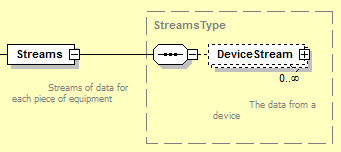
\includegraphics[width=1.0\textwidth]{figures/Streams Schema.png}
  \caption{Streams Schema Diagram}
  \label{fig:Streams Schema Diagram}
\end{figure}

\FloatBarrier


\begin{figure}[ht]
  \centering
    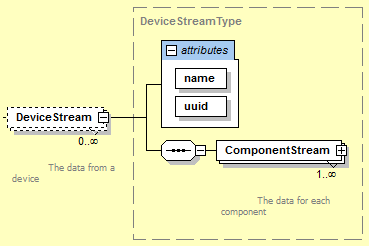
\includegraphics[width=1.0\textwidth]{figures/DeviceStream Schema.png}
  \caption{DeviceStream Schema Diagram}
  \label{fig:DeviceStream Schema Diagram}
\end{figure}

\FloatBarrier


\begin{figure}[ht]
  \centering
    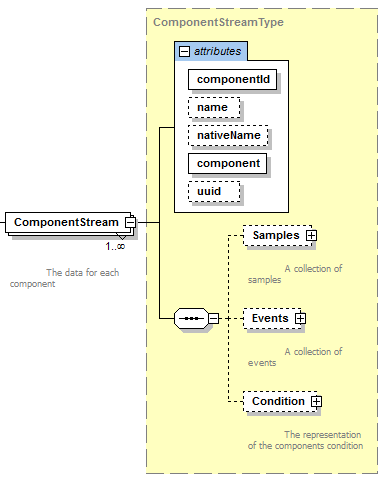
\includegraphics[width=1.0\textwidth]{figures/ComponentStream Schema.png}
  \caption{ComponentStream Schema Diagram}
  \label{fig:ComponentStream Schema Diagram}
\end{figure}

\FloatBarrier


\begin{figure}[ht]
  \centering
    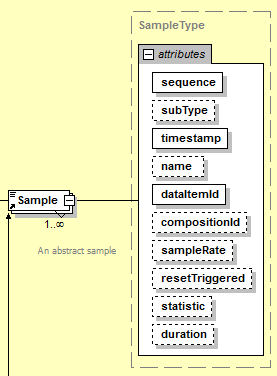
\includegraphics[width=1.0\textwidth]{figures/Sample Schema.png}
  \caption{Sample Schema Diagram}
  \label{fig:Sample Schema Diagram}
\end{figure}

\FloatBarrier


\begin{figure}[ht]
  \centering
    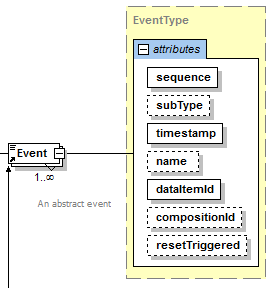
\includegraphics[width=1.0\textwidth]{figures/Event Schema.png}
  \caption{Event Schema Diagram}
  \label{fig:Event Schema Diagram}
\end{figure}

\FloatBarrier


\begin{figure}[ht]
  \centering
    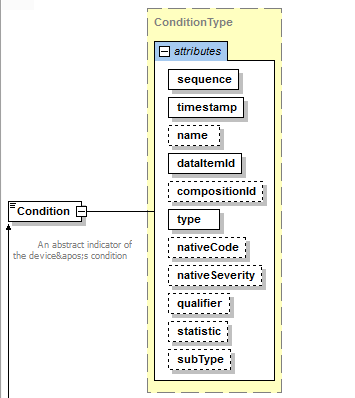
\includegraphics[width=1.0\textwidth]{figures/Condition Schema.png}
  \caption{Condition Schema Diagram}
  \label{fig:Condition Schema Diagram}
\end{figure}

\FloatBarrier


\subsubsection{Representation Schema Diagrams}
\label{sec:Representation Schema Diagrams}

\begin{figure}[ht]
  \centering
    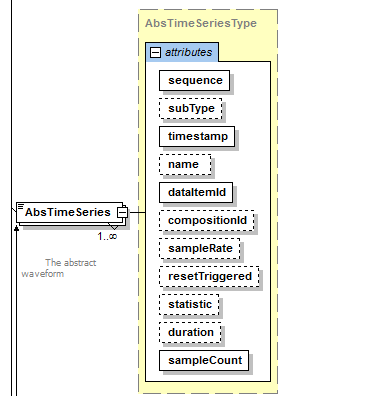
\includegraphics[width=1.0\textwidth]{figures/AbsTimeSeries Schema.png}
  \caption{AbsTimeSeries Schema Diagram}
  \label{fig:AbsTimeSeries Schema Diagram}
\end{figure}

\FloatBarrier


\begin{figure}[ht]
  \centering
    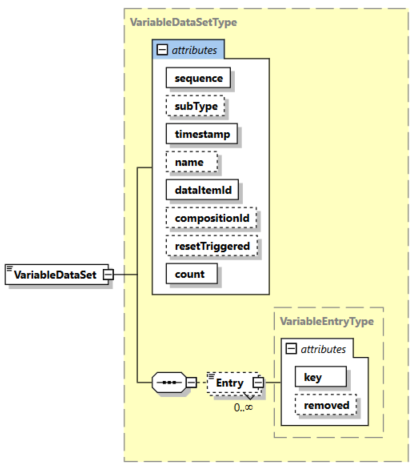
\includegraphics[width=1.0\textwidth]{figures/Sample DataSet Schema.png}
  \caption{Sample DataSet Schema Diagram}
  \label{fig:Sample DataSet Schema Diagram}
\end{figure}

\FloatBarrier


\begin{figure}[ht]
  \centering
    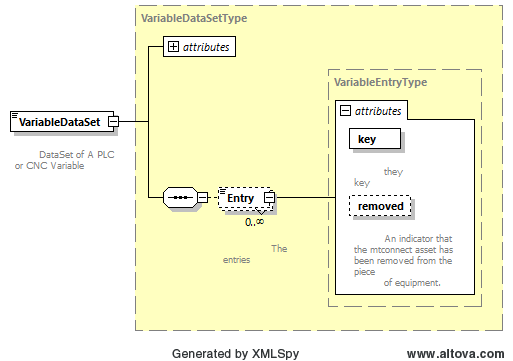
\includegraphics[width=1.0\textwidth]{figures/Entry Schema.png}
  \caption{Entry Schema Diagram}
  \label{fig:Entry Schema Diagram}
\end{figure}

\FloatBarrier


\begin{figure}[ht]
  \centering
    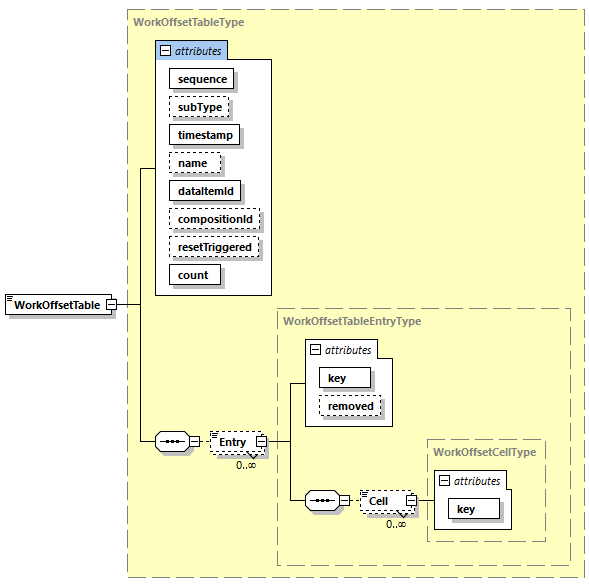
\includegraphics[width=1.0\textwidth]{figures/Table Schema.png}
  \caption{Table Schema Diagram}
  \label{fig:Table Schema Diagram}
\end{figure}

\FloatBarrier
